\section{Computation and critical phenomena}



%%%%%%%%%%%%%%%%%%%%%%%%%%%%%%%%%%%%%%%%%%%%%%%%%%%%%%%%%%
\begin{frame}[label=ladila]{The criticality view I}
 \begin{center}
  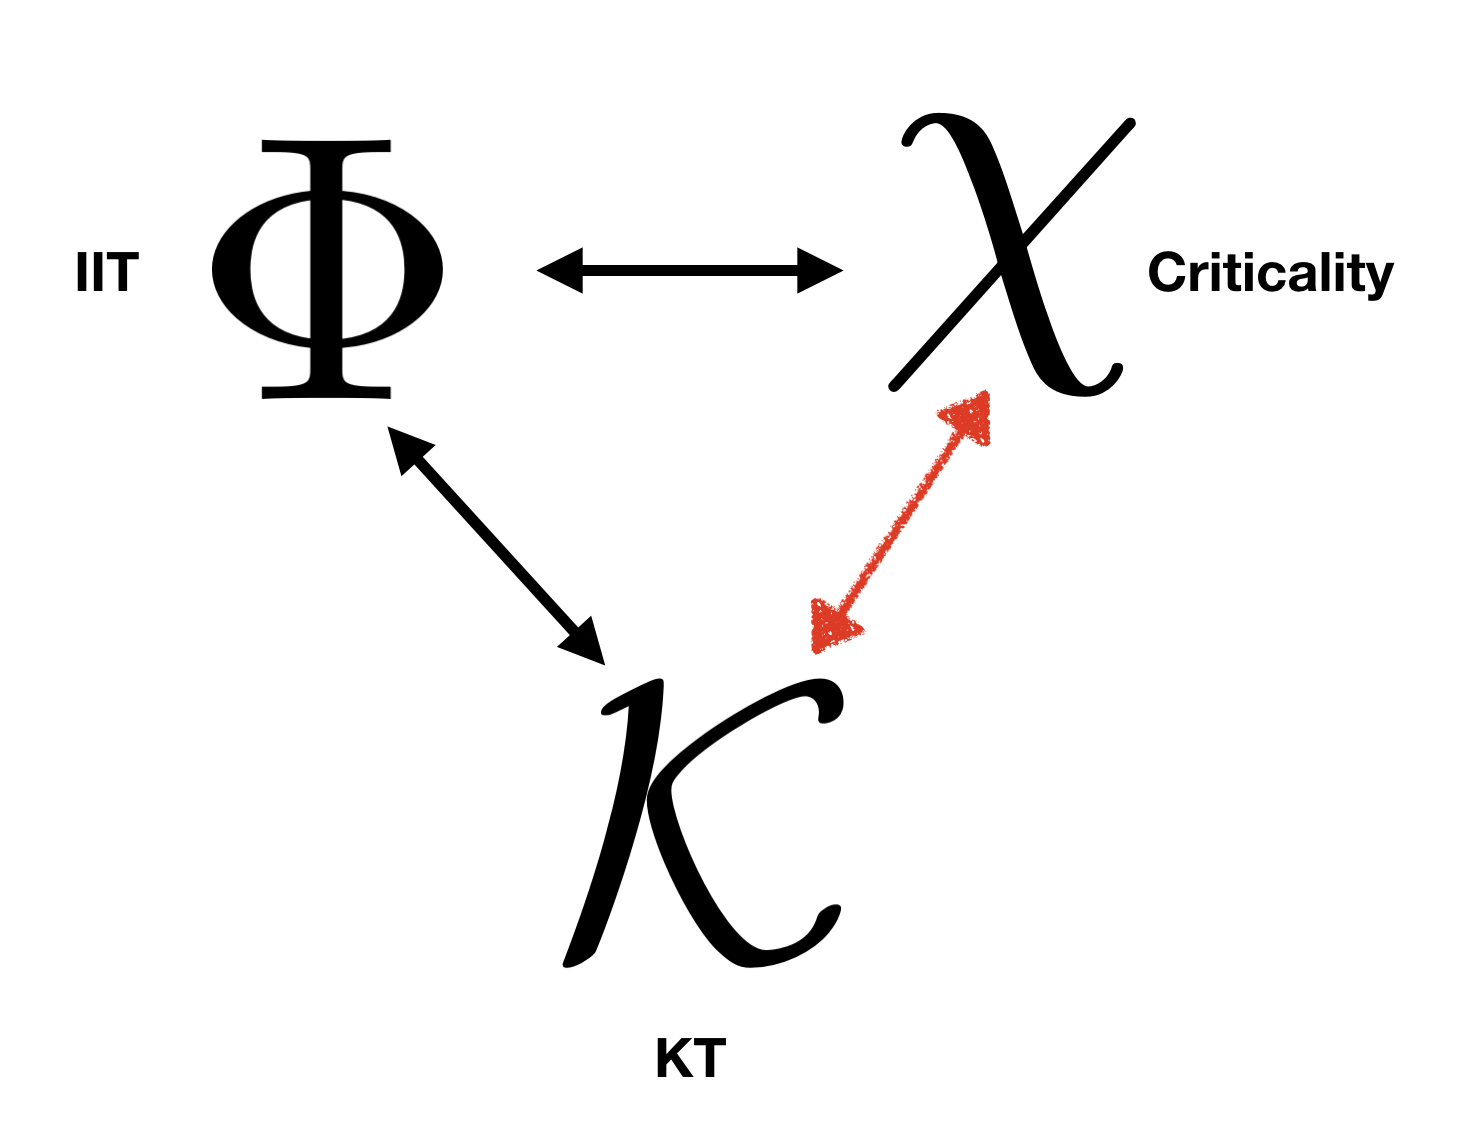
\includegraphics[height=8cm]{img/KUF.png}
  \end{center}
\end{frame}


%%%%%%%%%%%%%%%%%%%%%%%%%%%%%%%%%%%%%%%%%%%%%%%%%%%%%%%%%%
\begin{frame}[label=ladila]{The criticality view II}
 Computation  in Nature is carried out by dynamical systems with very large degrees of freedom.  \vfill
 
  Brains operate close to such critical boundaries consistent with the notion of self-organized criticality (SOC) \citep{Bak1988,Chialvo:2004aa,Cocchi2017,Carhart2018,Deco2021}. \vfill
  
  Altered state of consciousness appear to move the brain away or towards criticality \citep{CarhartHarris2019,Ruffini:2022ac}.  \vfill
  
  That KT and criticality theory  may be linked arises from the observation that  computational structures---dynamical systems---instantiating simple, compressive models of compositional data that exhibits regularities/symmetries (conserved quantities) must have special properties.  What are they?\vfill
 
  \end{frame}
  
  %%%%%%%%%%%%%%%%%%%%%%%%%%%%%%%%%%%%%%%%%%%%%%%%%%%%%%%%%%
  \begin{frame}[label=ladila]{The criticality view III}
  Recall the movie of a moving hand in empty space, $y(t) = f(\theta(t))$. %, where $y(t)$ represents the sequences of images of the hand as a function of parameters $\theta(t)$.
  \vfill
  
 Although $y$ may be embedded in a very high dimensional space, its dimension is actually very small if the set of parameters $\theta$ controlling the hand function is small.\vfill
  
The state of a dynamical system generating frames of the moving hand, regardless of how large its natural space is  (e.g., involving a large number of neurons) must also lie in a low dimensional subspace, a reduced manifold.  \vfill
  
   Ongoing work  on structured flow on manifolds \citep{Jirsa2020,Jirsa2022} highlights that near criticality (Re[$\lambda$]$\sim0$)the dynamics of complex systems collapse to low dimensional manifolds. 
   

\end{frame}

%%%%%%%%%%%%%%%%%%%%%%%%%%%%%%%%%%%%%%%%%%%%%%%%%%%%%%%%%%
\begin{frame}[label=ladila]{The criticality view IV---the center manifold}
A hand is a hand is a hand. 
 \begin{center}
  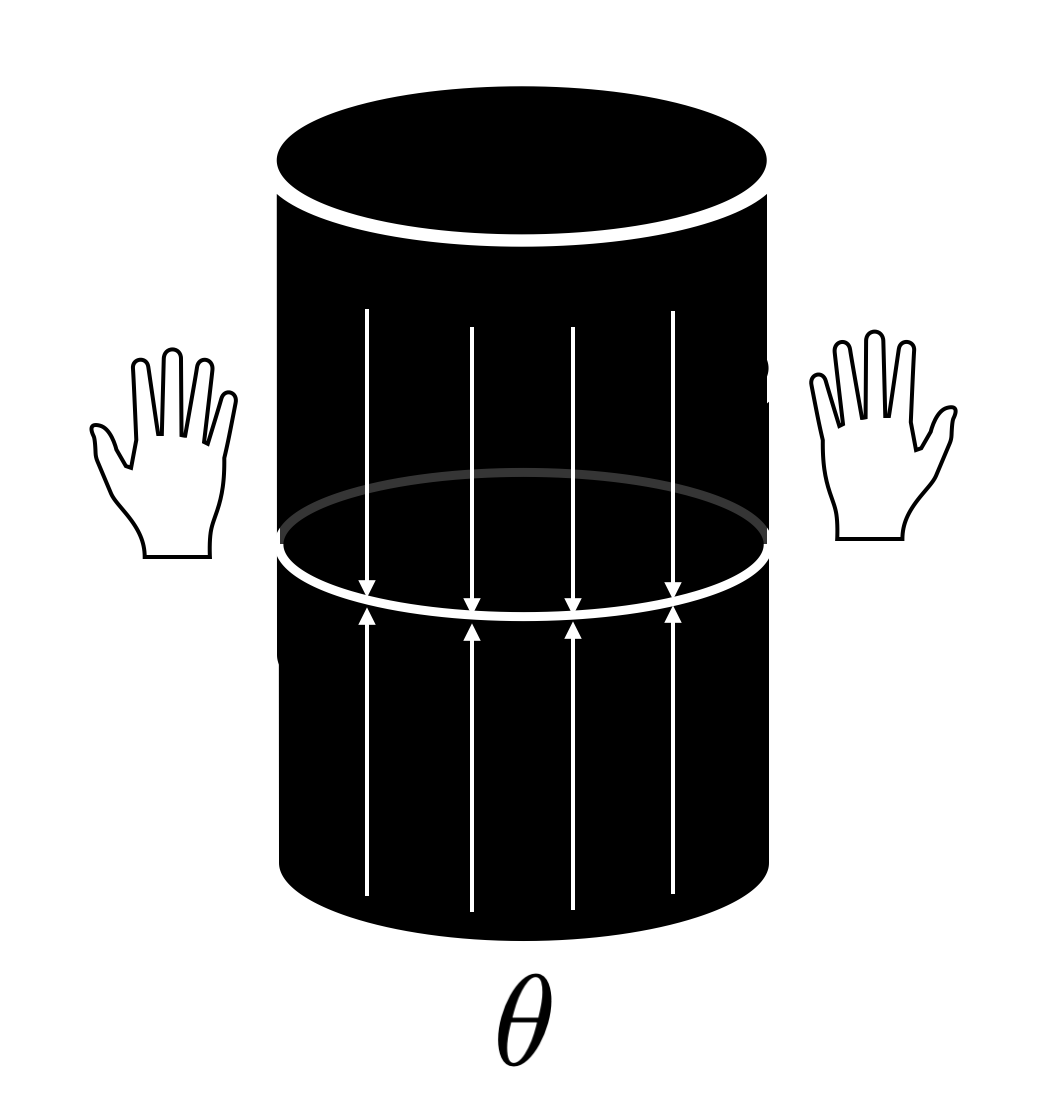
\includegraphics[height=6cm]{img/cylinder.png}
  \end{center}


\end{frame}



%%%%%%%%%%%%%%%%%%%%%%%%%%%%%%%%%%%%%%%%%%%%%%%%%%%%%%%%%%
\begin{frame}[label=ladila]{The criticality view V}

   Structure in data, the collapse of dynamics to low-dimensional spaces, criticality and associated features such as maximal information flow, power laws, long time scales and enhanced susceptibility,  \K and \SEP are thus deeply connected. \vfill 
   
The dimensionality and manifold structure of the reduced dynamics together with the mutual information of the system with the external world provide, respectively, metrics on the simplicity of the  models and the amount of algorithmic information captured.  \vfill


The structure of the reduced manifold maps into the structure of experience, while model accuracy and breath ($\mathcal M$) map into the realism and breath of experience.  These are the three dimensions of \SEP. \vfill

The agent-world lock loop, tracking real world (structured) data, helps to keep dynamics on the reduced manifold (\SEP!). Psychedelics, meditation, sensory deprivation may ``lift'' dynamics up from enslaved dynamics.

\end{frame}

